\documentclass[a4paper]{article}

%% Language and font encodings
\usepackage[utf8]{inputenc}
\usepackage[ngerman]{babel}
\usepackage[T1]{fontenc}

%% Sets page size and margins
\usepackage[a4paper,top=3cm,bottom=2cm,left=3cm,right=3cm,marginparwidth=1.75cm]{geometry}

%% Useful packages
\usepackage{amsmath}
\usepackage{graphicx}
\usepackage[style=nature]{biblatex}
\usepackage[colorinlistoftodos]{todonotes}
\usepackage[colorlinks=true, allcolors=blue]{hyperref}
\usepackage{float}

\addbibresource{references.bib}

\title{Praktikum Neurobiologie - Protokoll 1}

\author{Cedric Laier, Tilman Mehl}


\begin{document}
%Titelpage Modell: https://www.latextemplates.com/template/formal-book-title-page
\begin{titlepage} % Suppresses headers and footers on the title page

	\centering % Centre everything on the title page
	
	\scshape % Use small caps for all text on the title page
	
	\vspace*{\baselineskip} % White space at the top of the page
	
	%------------------------------------------------
	%	Title
	%------------------------------------------------
	
	\rule{\textwidth}{1.6pt}\vspace*{-\baselineskip}\vspace*{2pt} % Thick horizontal rule
	\rule{\textwidth}{0.4pt} % Thin horizontal rule
%	{\LARGE THE BIG BOOK\\ OF\\ \LaTeX ~TEMPLATES\\} % Title
	\vspace{0.75\baselineskip} % Whitespace above the title
	{\LARGE Elektromyogramm aus Insektenmuskeln\\} {Protokoll zum Praktikum Neurobiologie für Bioinformatiker\\ am 07.01.2019} % Title

	
	\vspace{0.75\baselineskip} % Whitespace below the title
	
	\rule{\textwidth}{0.4pt}\vspace*{-\baselineskip}\vspace{3.2pt} % Thin horizontal rule
	\rule{\textwidth}{1.6pt} % Thick horizontal rule
	
	\vspace{2\baselineskip} % Whitespace after the title block
	
	\vspace{2.0\baselineskip} % Whitespace before the editors

{\LARGE Gruppe 2}
\vspace{2.5\baselineskip} \\
	
{\LARGE Autoren:}
\begin{itemize}
\item Cedric Laier - \textit{cedric.laier@fu-berlin.de}
\item Tilman Mehl - \textit{tilmanmehl@zedat.fu-berlin.de}
\end{itemize}
\vspace{2.5\baselineskip}

{\LARGE Lehrveranstalter:}
\begin{itemize}
\item  Peter Robin Hiesinger
\item Matthias Wernet
\end{itemize}
\vspace{2.5\baselineskip}

{\LARGE Tutoren:}
\begin{itemize}
\item Lisa
\item Johannes
\item Claudia
\end{itemize}
	
\end{titlepage}


\section{Einleitung}
Inhalt des Praktikumstages war der Zusammenhang zwischen neuronaler Aktivität und Muskelaktivität. Konkret wurde die Muskelaktivität der Extensor Tibia einer Heuschrecke gemessen.\\
Wird ein (wirbelloses) Motoneuron innerviert, wird an den Synapsen zu den Muskelzellen Glutamat ausgeschüttet, was bei ausreichend hoher Konzentration zu einer Depolarisation der Muskelzellmembran und somit zu einer Muskelkontraktion führt.\\ \\
Die Messung dieser Spannungsänderungen nennt sich Elektromyogramm (EMG).\\
Es wurde jeweils ein EMG für ein Kick-Experiment, und ein Thrusting-Experiment angefertigt.\\
Beim Kick-Experiment wurde die Heuschrecke stimuliert, um mit ihrem Hinterbein eine vollständige Streckung auszuführen. \\ \\
Beim Thrusting-Experiment wurde die gleiche Bewegung stimuliert, allerdings wurde die vollständige Streckung mit Hilfe eines Stifts blockiert.

\section{Versuchsaufbau und -durchführung}

\subsection{Versuchsaufbau}
Für die Messung der Aktionspotentiale wurde eine extrazelluläre differentielle Ableitung vorgenommen. Dazu wurden zwei Drahtelektroden nah aneinander in die Tibia der Heuschrecke gesteckt. Die extrazellulär gemessenen Ströme sind sehr gering und es musste ein Differenzverstärker verwendet werden, um diese sichtbar zu machen. Durch zusätzliche Hoch- und Tiefpassfilter konnten unerwünschte Frequenzbereiche aus unserem Strom gefiltert werden. Ein an den Differenzverstärker angeschlossener Analog-Digital-Wandler erlaubte das analoge Signal für den PC digital umzuwandeln, sodass wir mithilfe von dem Programm Spike2 \cite{Spike2:Online} in der Lage waren das EMG Signal aufzeichnen, darstellen und auswerten zu können. Abbildung 1 skizziert den genannten Versuchsaufbau.

\subsection{Versuchskizze} 
\vspace{2.5\baselineskip}
\begin{figure}[H]
    \centering
    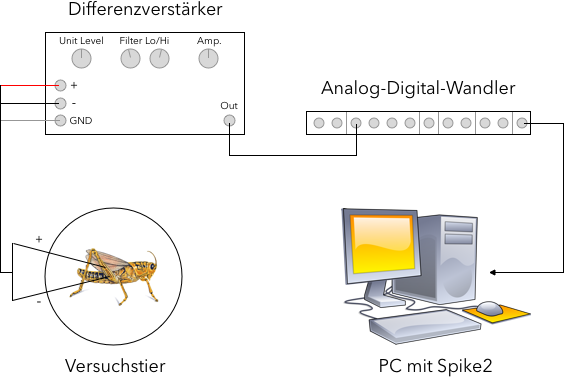
\includegraphics[scale=0.6]{images/Versuchsaufbau.png}
    \caption{Skizze des Versuchaufbaus}
\end{figure}


\newpage
\subsection{Versuchsdurchführung}
Im Rahmen des Experimentes wurden zwei unterschiedliche Messungen vorgenommen. Die erste Messung erfolgte bei dem sogenannten \texttt{Kick} Verhalten der Heuschrecke, die zweite Messung bei dem \texttt{Thrusting} Verhalten. Um die Messung an der Heuschrecke durchführen zu können, wurde die Heuschrecke mithilfe von Knete in Rückenlage auf einem Trägerbrett fixiert, sodass diese nur noch eines ihrer Sprungbeine bewegen konnte. An diesem Sprungbein wurden zwei Drahtelektroden, mit ein wenig Abstand voneinander, im Muskel der Heuschrecke versenkt.  
\subsubsection{Kick Messung}
Mithilfe von einem Pinsel wurde die Heuschrecke stimuliert, um einen Tritt zu erzwingen. Wir wiederholten diesen Vorgang während der Aufzeichnung so lange, bis wir eine zufriedenstellende Freqeuenzmessung mit zwei gut erkennbaren Aktionpotentialen aufzeichnen konnten. 

\subsubsection{Thrusting Messung}
Auch hier wurde ein \texttt{Kick} Verhalten mithilfe vom Pinsel forciert. Allerdings erweiterten wir diese Messung, in dem wir den Streckbereich des Beines auf halbem Wege mit einem Bleistift blockierten. Dieser Schritt wurde erneut so oft wiederholt, bis wir gut erkennbare Messungen aufzeichnen konnten.

\section{Ergebnisse}

\subsection{Kick-EMG}

Beim Kick-EMG wurde eine Frequenz von 3 Hz beobachtet. \\
Die beiden Amplitudenmessungen hatten eine Amplitudenhöhe von -0,221 V bzw. 0,170 V und Amplitudendauer von 10 ms bzw. 11 ms.

\vspace{2.5\baselineskip}
\begin{figure}[H]
    \centering
        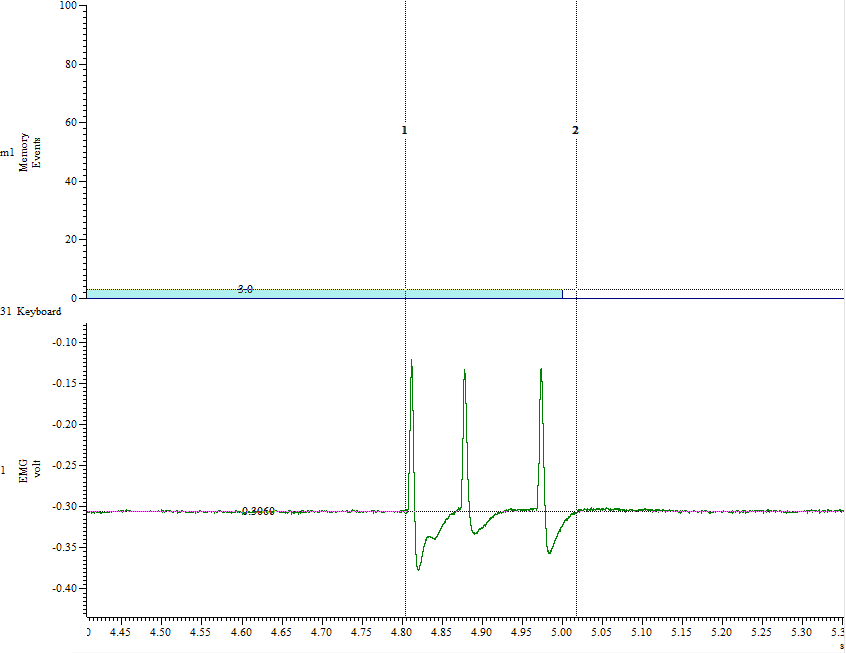
\includegraphics[scale=0.5]{images/kick_freq.png}
    \caption{Frequenz Kick-EMG}
\end{figure}

\begin{figure}[H]
    \centering
        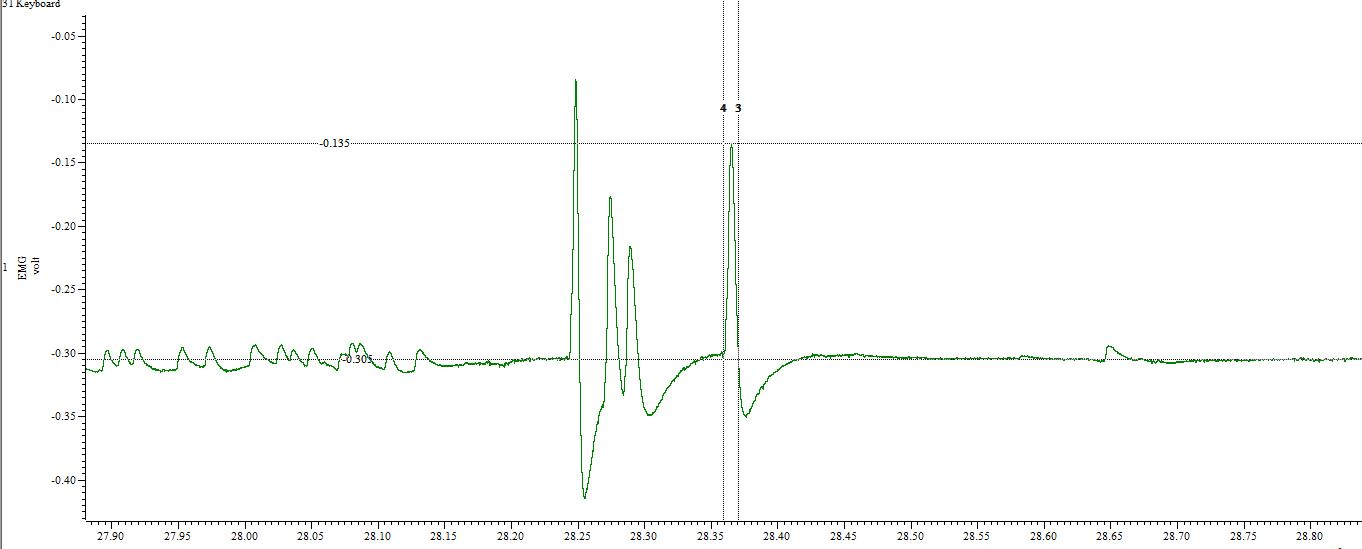
\includegraphics[scale=0.35]{images/kick.JPG}
    \caption{Amplitudenhöhe Kick-EMG}
\end{figure}


\subsection{Thrusting-EMG}
Beim Thrusting-EMG wurde eine durchschnittliche Frequenz von 7,3 Hz beobachtet. \\
Die beiden Amplitudenmessungen hatten jeweils eine Amplitudenhöhe von -0,158 V und Amplitudendauer von 10 ms.
\vspace{2.5\baselineskip}
\begin{figure}[H]
    \centering
    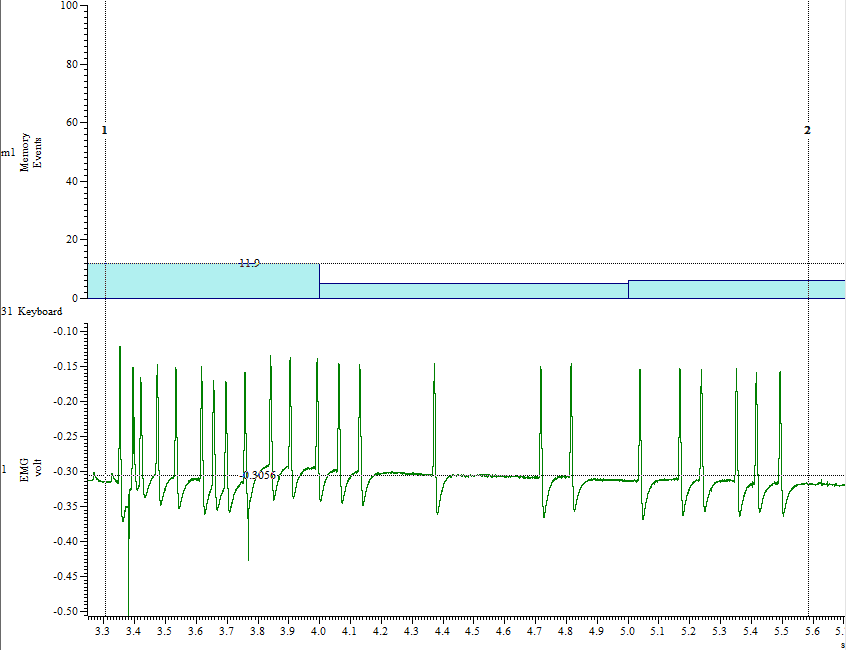
\includegraphics[scale=0.5]{images/thrusting_freq.png}
    \caption{Frequenz Thrusting-EMG}
\end{figure}
\begin{figure}[H]
    \centering
    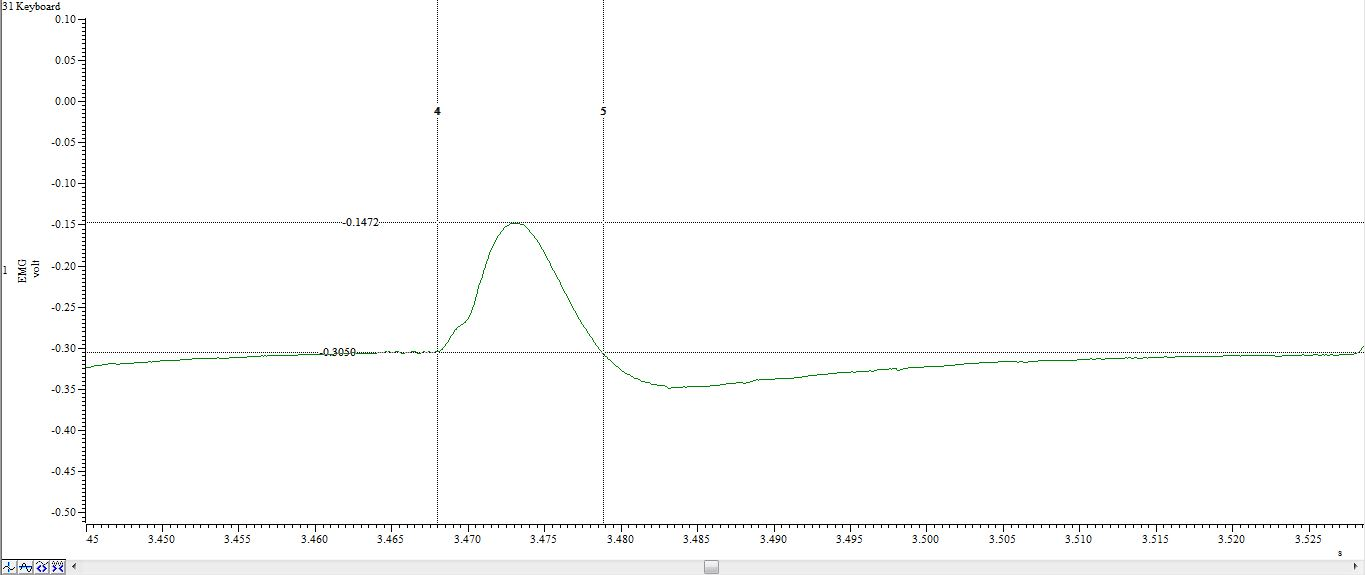
\includegraphics[scale=0.35]{images/thrusting.JPG}
    \caption{Amplitudenhöhe Thrusting-EMG}
\end{figure}

\section{Diskussion}

Beim \texttt{Kick} konnte man wie erwartet Aktionspotentiale und dazugehörige Muskelaktivität beobachten. \\
Beim \texttt{Thrusting} konnte man den Widerstandsreflex beobachten. Das Chordontonalorgan im Heuschreckenbein misst, ob der Streckermuskel die korrekte Länge erreicht hat, also das Bein vollständig gestreckt ist. Solange dies nicht der Fall ist, werden Aktionspotentiale generiert, um das Bein vollständig zu strecken. 

\printbibliography

\end{document}